\chapter{HASIL DAN PEMBAHASAN}

% Ubah bagian-bagian berikut dengan isi dari pengujian dan analisis

Pada bab ini dipaparkan hasil dan analisa dari pelaksanaan tiap tahap pada metodologi, skenario pengujian dan evaluasi pengujiannya. Pengujian dan evaluasi dilakukan guna mengetahui tingkat kesalahan dalam metodologi serta ananlisis untuk mencapai kesimpulan.Tahapan scenario pengujian meliputi hal berikut :

\begin{enumerate}
  \item Pengujian akurasi model dalam beberapa situasi
  \item Pengujian interaksi model pada beberapa responden
  \item Pengujian pada robot dengan beberapa kondisi
\end{enumerate}
Dengan hasil metodologi serta pelaksanaan skenario-skenario pengujian yang dipaparkan pada bab Penelitian dan pembahasan, diharapkan mendapatkan hasil dan analisa sehingga dapatditarik kesimpulan dari pelaksanaan tugas akhir ini.

\section{Hasil metodologi}
Pada metodologi terdapat blok diagaram sebagai acuan dalam Penelitian yang telah dilaksanakan. Adapun hasil dari blok diagram tersebut secara rinci sebagai berikut :

\subsection{Hasil dataset}
Proses pengumpulan dataset dilakukan dengan pengambilan citra menggunakan kamera. Proses tersebut dilakukan selama beberapa waktu untuk dapat mendapatkan beberapa frame citra untuk suatu class dan diulang kembali dengan class yang berbeda sampai seluruh class terpenuhi. Seluruh citra tangan diambil dari satu orang yang sama dan menggunakan jarak pengambilan yang sama, yaitu jarak antara kamera dan tangan. Dalam proses pengambilan citra dilakukan beberapa variasi dalam pose tangan yaitu dengan sedikit merotasikan tangan dan sedikit melemaskan tangan. Hal ini dilakukan agar tiap class memiliki variasi pose dan dapat mendeteksi dari berbagai kondisi pose. Adapun pose yang digunakan sebagai dataset dapat dilihat pada Tabel \ref{tab:citradaset}.

\begin{table}[H]
  \centering
  \caption{Citra hasil dataset}
  \label{tab:citradaset}
  \begin{tabular}{|c|c|}
  \hline
  Pose   & Citra \\ \hline
  Diam   & 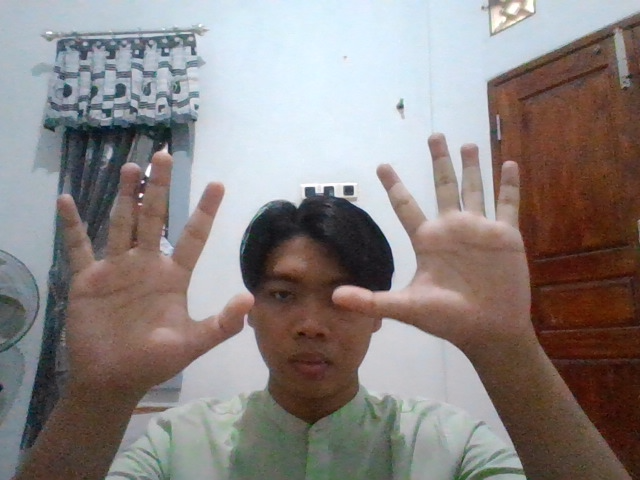
\includegraphics[width=0.3\linewidth]{gambar/posediam.png} \\ \hline
  Kanan  & 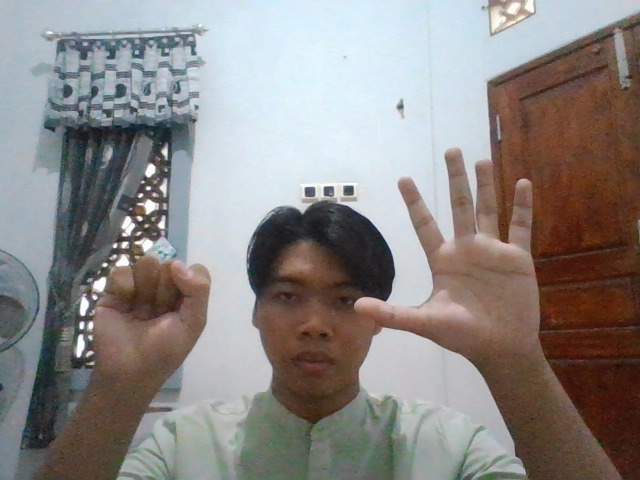
\includegraphics[width=0.3\linewidth]{gambar/posekanan.png} \\ \hline
  Kiri   & 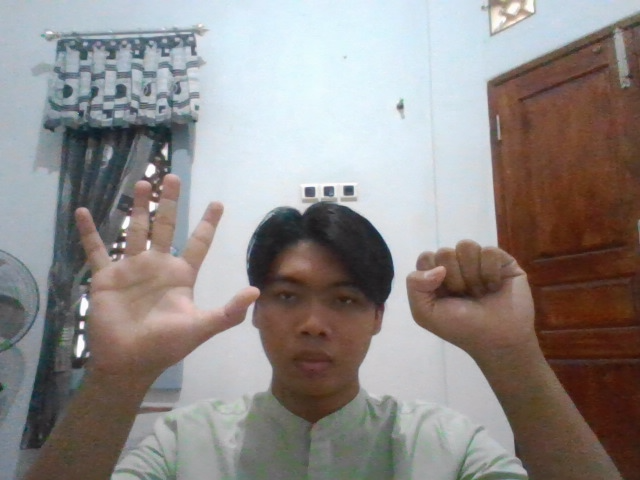
\includegraphics[width=0.3\linewidth]{gambar/posekiri.png} \\ \hline
  Maju   & 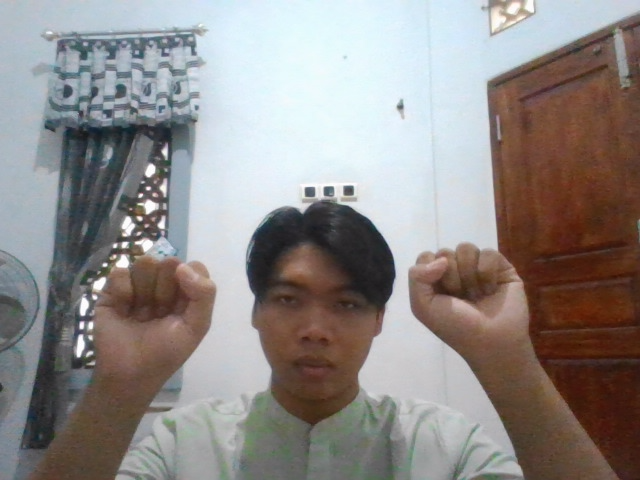
\includegraphics[width=0.3\linewidth]{gambar/posemaju.png} \\ \hline
  Mundur & 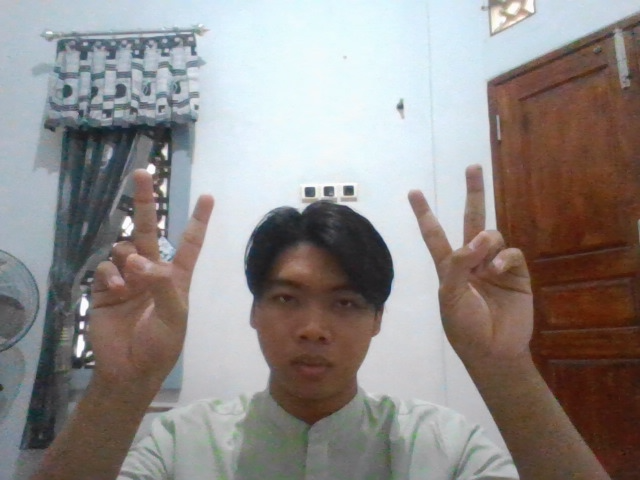
\includegraphics[width=0.3\linewidth]{gambar/posemundur.png} \\ \hline
  Tembak & 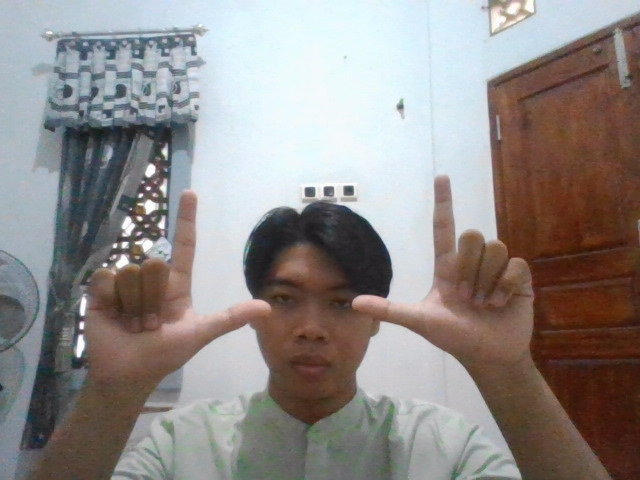
\includegraphics[width=0.3\linewidth]{gambar/posetembak.png} \\ \hline
\end{tabular}
\end{table}


\subsection{Hasil Pose \emph{Prediction}}

\begin{figure}[H]
  \centering
  \begin{tabular}{cc}
    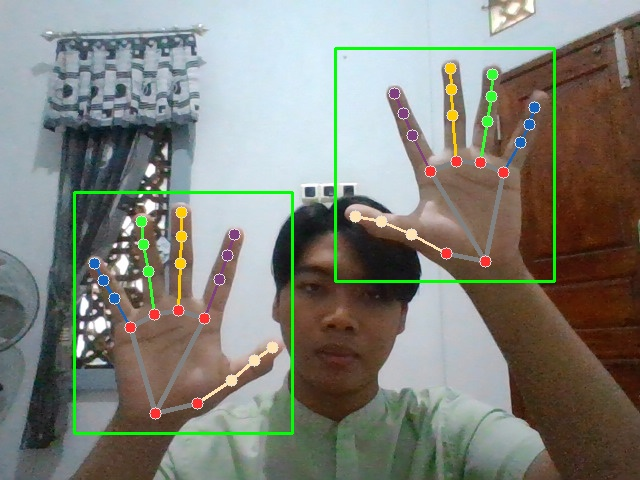
\includegraphics[width=0.4\linewidth]{gambar/hasilposepred.jpg} & 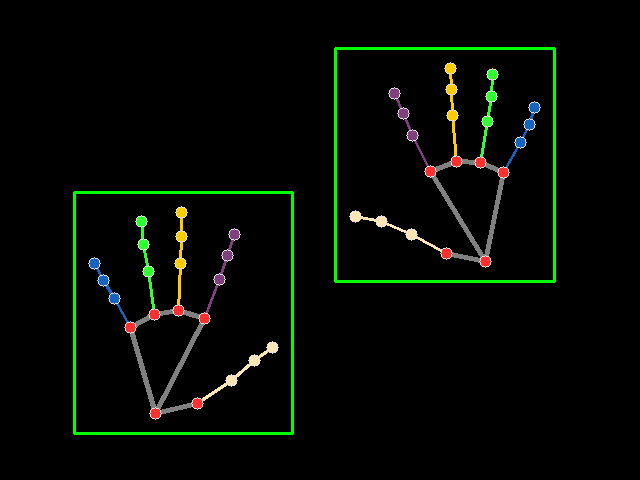
\includegraphics[width=0.4\linewidth]{gambar/hasilposepredhitam.png} \\
    a. Citra berwarna & b. Citra hitam 
    \end{tabular}
    \caption{Hasil\emph{ hand landmark}}
  \label{fig:hasilposepred}
\end{figure}

Proses pose \emph{prediction} dilakukan dengan menggambar \emph{hand landmark} yang telah terdeteksi dengan menggunakan \emph{Mediapipe} pada tiap-tiap citra yang telah dikumpulan pada tahap sebelumnya. Setelah \emph{hand landmark} tergambar maka tiap-tiap \emph{hand landmark} digambar pada citra berlatar gelap. Hasil dari \emph{hand landmark} pada citra hasil kamera dan citra hitam dapat dilihat pada Gambar \ref{fig:hasilposepred}. \emph{Hand landmark} yang terdapat pada citra ini diberikan \emph{bounding box} pada tiap tangan. Setelah \emph{bounding box} terbuat maka selanjutnya dilakukan \emph{hand localization} pada \emph{hand landmark} yang berada pada citra hitam. \emph{Hand} \emph{localization} ini untuk mengecilkan ukuran citra menjadi hanya selebar \emph{bounding box} dengan ditambah 20 \emph{pixel} pada nilai maksimal dan dikurangi 20 \emph{pixel} pada nilai minimum pada tiap \emph{bounding box}. Penambahan \emph{pixel} ini dimaksudkan untuk mencakup semua \emph{hand landmark} yang telah dibuat \emph{Mediapipe}. Dengan mengurangi ukuran citra ini bertujuan mengurangi waktu training dan dapat meningkatkan performa. Citra diluar \emph{bounding box} dibuang dan tiap \emph{bounding box} dirubah ukurannya menjadi 128x128 \emph{pixel} untuk menyamakan kedua \emph{bounding box} dalam satu frame citra. Setelah setiap ukuran \emph{bounding box} sama maka setiap \emph{bounding box} ditumpuk secara horizontal. Citra yang disimpan dan dijadikan dataset adalah citra yang terdapat dua \emph{hand landmark} yang telah ditumpuk secara horizontal. Citra yang disimpan nantinya memiliki ukuran 256x128 \emph{pixel} dikarenakan hasil dari dua tangan yang terdeteksi. Pada tahap menumpuk citra terdapat dua macam tumpukan yaitu citra dengan posisi tangan kiri berada pada kotak sebelah kiri dan tangan kanan pada kotak sebelah kanan. Posisi kedua yaitu tangan kiri berada pada posisi kanan dan tangan kanan berada pada kiri yang selanjutnya disebut sebagai posisi invers. Posisi \emph{hand landmark} dari hasil hand localization dapat dilihat pada Tabel \ref{tab:posisigtangan}.

\begin{table}[H]
  \centering
  \caption{Hasil posisi hand localization}
  \label{tab:posisigtangan}
  \begin{tabular}{|c|c|c|}
  \hline
  Pose   &Pose Benar&Pose Invers\\ \hline
  Diam   & 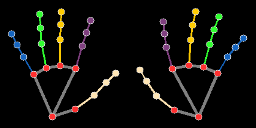
\includegraphics[width=0.3\linewidth]{gambar/Diam (1).png} & 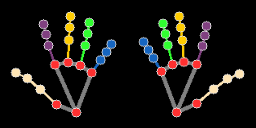
\includegraphics[width=0.3\linewidth]{gambar/DiamI (1).png} \\ \hline
  Kanan  & 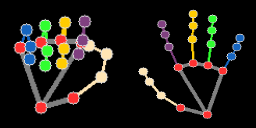
\includegraphics[width=0.3\linewidth]{gambar/Kanan (1).png} & 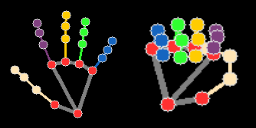
\includegraphics[width=0.3\linewidth]{gambar/KananI (1).png} \\ \hline
  Kiri   & 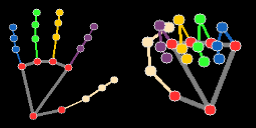
\includegraphics[width=0.3\linewidth]{gambar/Kiri (1).png} & 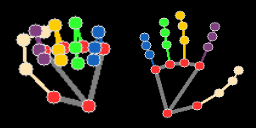
\includegraphics[width=0.3\linewidth]{gambar/KiriI (1).png} \\ \hline
  Maju   & 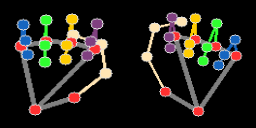
\includegraphics[width=0.3\linewidth]{gambar/Maju (1).png} & 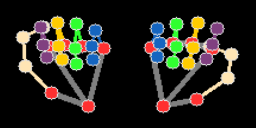
\includegraphics[width=0.3\linewidth]{gambar/MajuI (1).png} \\ \hline
  Mundur & 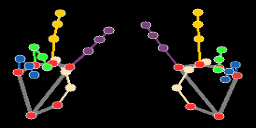
\includegraphics[width=0.3\linewidth]{gambar/Mundur (1).png} & 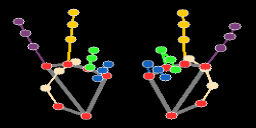
\includegraphics[width=0.3\linewidth]{gambar/MundurI (1).png} \\ \hline
  Tembak & 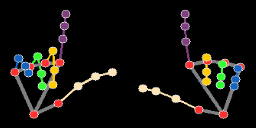
\includegraphics[width=0.3\linewidth]{gambar/Tembak (1).png} & 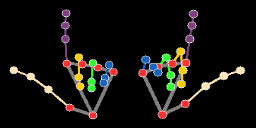
\includegraphics[width=0.3\linewidth]{gambar/TembakI (1).png} \\ \hline
  \end{tabular}
\end{table}




\subsection{Hasil \emph{Classification}}
Proses classification dimulai dari \emph{training} dataset. Sebelum melakukan \emph{training} maka dibutuhkannya data citra pada tiap class. Tiap class memiliki \emph{train data} dan \emph{validation data}. Data-data ini diambil dari proses sebelumnya yaitu citra yang telah melewati tahap hand localization. Citra untuk train data pada tiap class berjumlah 400 dengan rincian 200 citra posisi benar dan 200 citra posisi invers, sedangkan citra untuk \emph{validation data} berjumlah 80 citra dengan 40 citra posisi benar dan 40 citra posisi invers. Adapaun tabel pesebaran data citra tiap class dapat dilihat pada Tabel \ref{tab:tiapclass}. \emph{Training} ini menggunakan CNN dengan menggunakan satu layer \emph{convolution} ukuran 3x3 dengan filter 16, sehingga ukuran citra yang awalnya 256x128 turun menjadi 254x126 yang disebabkan dari adanya konvolusi. Selanjutnya dilakukan \emph{pooling} dengan menggunakan \emph{max} \emph{pooling} ukuran 2x2 yang menyebabkan ukuran citra turun menjadi setengah dari hasil konvolusi yaitu 167x63. Layer selanjutnya yaitu \emph{flatten} dimana citra hasil dari max pooling di ubah menjadi vektor. Output yang didapatkan dari layer \emph{flatten} yaitu 128016 vektor.  Setelah di tentukannya konfigurasi layer CNN maka tahapan selanjutnya yaitu konfigurasi hyperparameter. Adapun konfigurasi pada hyperparameter yang digunakan dapat dilihat pada Tabel \ref{fig:hyperparameter} berikut.

\begin{table}[H]
  \centering
  \caption{Jumlah Citra Tiap \emph{Class}}
  \label{tab:tiapclass}
  \begin{tabular}{|c|c|c|}
  \hline
  \emph{Class}  & Train Data & Validation Data \\ \hline
  Diam   & 400        & 80              \\ \hline
  Kanan  & 400        & 80              \\ \hline
  Kiri   & 400        & 80              \\ \hline
  Maju   & 400        & 80              \\ \hline
  Mundur & 400        & 80              \\ \hline
  Tembak & 400        & 80              \\ \hline
  \end{tabular}
\end{table}

\begin{table}[H]
  \centering
  \caption{Konfigurasi \emph{hyperparameter}}
  \label{fig:hyperparameter}
  \begin{tabular}{|c|c|lll}
  \cline{1-2}
  \emph{Hyperparameter} & Konfigurasi \\ \cline{1-2}
  Epochs         & 20 \\ \cline{1-2}
  Batchsize      & 32 \\ \cline{1-2}
  Image Size     & 256x128 \\ \cline{1-2}
  Step per epoch      & 75 \\ \cline{1-2}
  Optimizer      & Adam \\ \cline{1-2}
  \end{tabular}
\end{table}

Setelah proses konfigurasi layer CNN dan \emph{hyperparameter} telah dilakukan. Selanjutnya yaitu proses \emph{training} yaitu berupa model dan detail data pada tiap proses pengulangan. Hasil dari \emph{training} ini didapatkan \emph{training} \emph{accuracy}, \emph{validation} \emph{accuracy}, \emph{training} \emph{loss}, dan \emph{validation} \emph{loss}. Setiap perulangan mendapatkan nilai tersebut, grafik dari nilai tersebut dalam 20 perulangan dapat dilihat pada Gambar \ref*{fig:loss} dan Gambar \ref*{fig:akurasi}

\begin{figure}[H]
  \centering
  \includegraphics[width=0.7\linewidth]{gambar/loss.png}
  \caption{Grafik \emph{training} dan \emph{validation} \emph{loss}}
  \label{fig:loss}
\end{figure}

\begin{figure}[H]
  \centering
  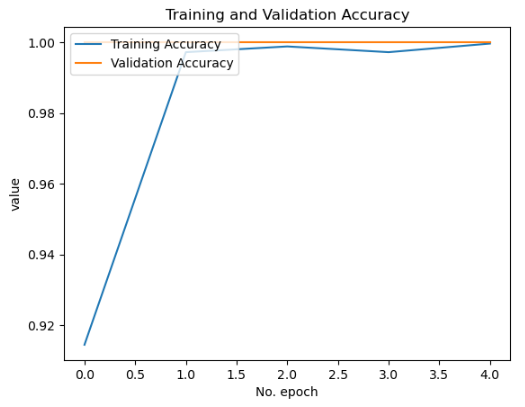
\includegraphics[width=0.7\linewidth]{gambar/akurasi.png}
  \caption{Grafik \emph{training} dan \emph{validation} \emph{accuracy}}
  \label{fig:akurasi}
\end{figure}

Setelah proses \emph{training} selesai dan telah didapatkan model dengan akurasi yang tinggi atau sesuai \emph{threshold} dalam hal ini dapat dilihat pada grafik akurasi pada Gambar \ref{fig:akurasi}, maka selanjutnya masuk kepada proses evaluasi model. Evaluasi model menggunakan \emph{confusion matrix} dengan data testing citra sebanyak 100 pada masing-masing class. Hasil dari \emph{confusion matrix} didapatkan akurasi 0.95. Hasil evaluasi dengan \emph{confusion matrix} secara lengkap dapat dilihat pada Gambar \ref{fig:confusionmatrix}. Model yang telah dievaluasi menggunakan \emph{confusion matrix} selanjutnya digunakan sebagai \emph{classification}. \emph{Classification} menghasilkan kode instruksi yang digunakan sebagai acuan dalam memberikan perintah kepada robot. Adapun kode instruksi yang diatur sebagai perintah kepada robot dapat dilihat pada Tabel \ref{tab:kodeinstruksi}

\begin{figure}[H]
  \centering
  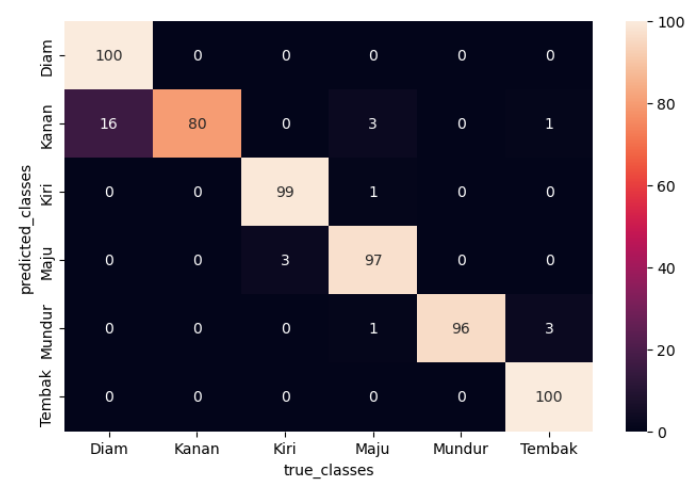
\includegraphics[width=0.7\linewidth]{gambar/confusionmatrix.png}
  \caption{Hasil \emph{Confusion Matrix}}
  \label{fig:confusionmatrix}
\end{figure}

\begin{table}[H]
  \centering
  \caption{Kode instruksi hasil \emph{classification}}
  \label{tab:kodeinstruksi}
  \begin{tabular}{|c|c|}
  \hline
  Pose   & Kode Instruksi \\ \hline
  Diam   & n              \\ \hline
  Kanan  & r              \\ \hline
  Kiri   & l              \\ \hline
  Maju   & f              \\ \hline
  Mundur & b              \\ \hline
  Tembak & s              \\ \hline
  \end{tabular}
\end{table}

\subsection{\emph{Control Navigation}}
Proses \emph{control navigation} diawali dengan perancangan pada robot. Robot dirancang dengan memiliki kemampuan untuk bergerak dan menembak. Pergerakan robot dapat terjadi dikarenakan adanya sepasang roda yang dipasangkan pada robot. Perputaran roda diatur dari motor driver dengan menyalurkan listrik kepada motor dc yang sudah dipasangkan roda sebagai outputya. Kemampuan menembak pada robot diatur dengan adanya sensor \emph{infrared}. Sensor \emph{infrared transmitter} diletakkan didepan robot sedangakn sensor \emph{infrared receiver} membutuhkan empat yang diletakkan disekeliling sisi robot. Sensor infrared receiver akan di sambungkan secara pararel untuk ke empat sensornya dan dihubungkan kepada mikrokontroler dalam hal ini yang digunakan adalah "nodeMCU ESP8266". Secara schematic dapat dilihat pada Gambar \ref{fig:schematic}. Robot yang telah dirancang selanjutnya diuji dengan cara mengirimkan kode instruksiyang dihasilkan dari proses \emph{classification} kepada mikrokontroler robot. Pengujian ini dilakukan dengan mengklasifikasi 20 citra pada tiap class. Pengujian ini bertujuan untuk mengetahuiapakah ada data yang tidak terkirim atau hilang saat dikirim. Hasil dari klasifikasi akan dirubah menjadi kode instruksi dan dikirim kepada mikrokontroler. Pada mikrokontroler dihitung jumlah kode instruksi yang masuk dan dibandingkan dengan kode yang dikirim. Hasil pengujian ini dapat dilihat pada Tabel \ref{tab:hasulujipose}

\begin{table}[H]
  \centering
  \caption{Hasil uji komunikasi laptop dengan robot}
  \label{tab:hasulujipose}
  \begin{tabular}{|c|c|}
  \hline
  Pose   &  Hasil Uji\\ \hline
  Diam   & 20              \\ \hline
  Kanan  & 20             \\ \hline
  Kiri   & 20              \\ \hline
  Maju   & 20              \\ \hline
  Mundur & 20              \\ \hline
  Tembak & 20              \\ \hline
  \end{tabular}
\end{table}

\begin{figure}[H]
  \centering
  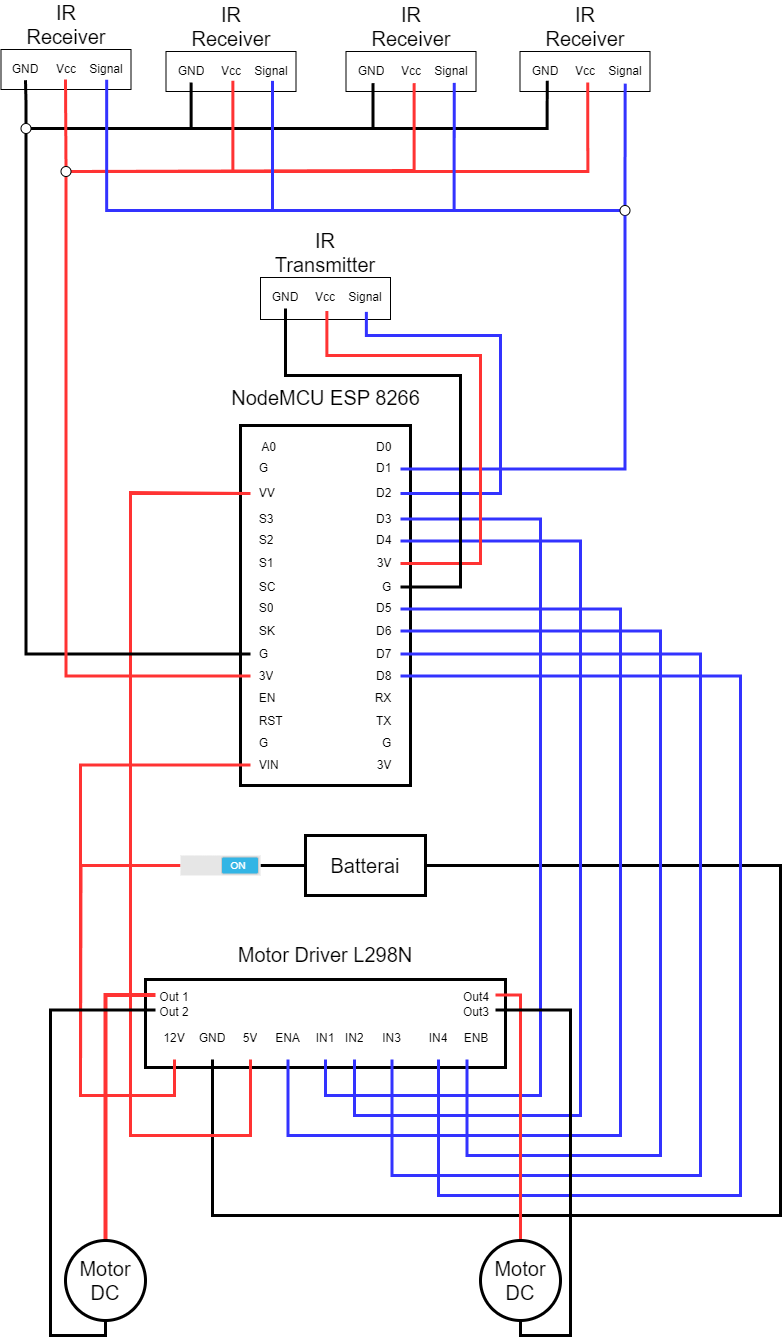
\includegraphics[width=0.5\linewidth]{gambar/schematic.png}
  \caption{\emph{Schematic} robot}
  \label{fig:schematic}
\end{figure}

\section{Skenario pengujian}
Pada skenario pengujian dilakukan beberapa skenario pengujian untuk mengetahui tingkat kesalahan dan membuka potensi pengembangan penelitian serta menarik kesimpulan secara keseluruhan. Skenario pegujian yang dilakukan yaitu sebagai berikut :
\subsection{Pengujian akurasi model}
Pengujian akurasi model bertujuan untuk membandingkan akurasi model dalam beberapa situasi uji guna mengetahui situasi ideal untuk melakukan classification. Pengujian ini menggunakan tangan peneliti dengan variasi jarak tangan terhadap kamera, intensitas cahaya ruangan, dan sudut kamera terhadap tangan. Hasil dari pengujian tersebut secara spesifik sebagai berikut :
\begin{enumerate}
  \item Pengujian jarak \\
  Pengujian jarak dilakukan dengan cara mengambil 20 citra dari tiap \emph{class} pada jarak tertentu. Jarak ini dimulai dari 30cm, 50cm, dan 100cm antara tangan dengan kamera. Pengujian dilakukan karena adanya perubahan bentuk dari \emph{hand landmark}. Hasil pose yang terdeteksi dari pengujian jarak dapat dilihat pada Tabel \ref{tab:hasiljarak}

  \begin{table}[H]
    \centering
    \caption{Pose yang terdeteksi dari pengujian jarak}
    \label{tab:hasiljarak}
    \begin{tabular}{|c|clll|}
      \hline
      \multirow{2}{*}{Pose} & \multicolumn{4}{c|}{Jarak (cm)}                                                   \\ \cline{2-5} 
                            & \multicolumn{1}{l|}{30} & \multicolumn{1}{l|}{50} & \multicolumn{1}{l|}{80} & 100 \\ \hline
      Diam                  & \multicolumn{1}{c|}{20}   & \multicolumn{1}{l|}{19}   & \multicolumn{1}{l|}{20}   &   20  \\ \hline
      Kanan                 & \multicolumn{1}{c|}{20}   & \multicolumn{1}{l|}{20}   & \multicolumn{1}{l|}{16}   &   10  \\ \hline
      Kiri                  & \multicolumn{1}{c|}{19}   & \multicolumn{1}{l|}{20}   & \multicolumn{1}{l|}{20}   &   20  \\ \hline
      Maju                  & \multicolumn{1}{c|}{19}   & \multicolumn{1}{l|}{20}   & \multicolumn{1}{l|}{20}   &   20  \\ \hline
      Mundur                & \multicolumn{1}{c|}{20}   & \multicolumn{1}{l|}{20}   & \multicolumn{1}{l|}{20}   &   20  \\ \hline
      Tembak                & \multicolumn{1}{c|}{20}   & \multicolumn{1}{l|}{20}   & \multicolumn{1}{l|}{15}   &   10  \\ \hline
      Akurasi                  & \multicolumn{1}{c|}{0.95}   & \multicolumn{1}{l|}{0.99}   & \multicolumn{1}{l|}{0.93}   &   0.83  \\ \hline
    \end{tabular}
  \end{table}

  \begin{figure}[H]
      \begin{tabular}{cccc}
        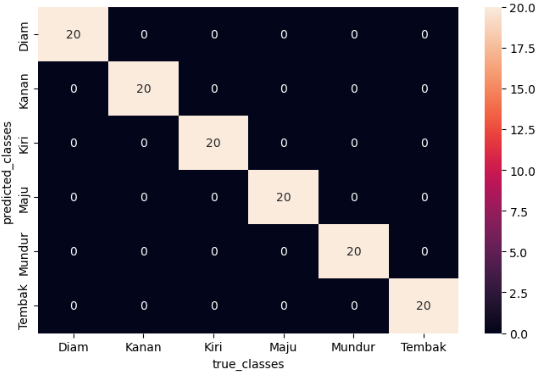
\includegraphics[width=0.4\linewidth]{gambar/cm30.png} & 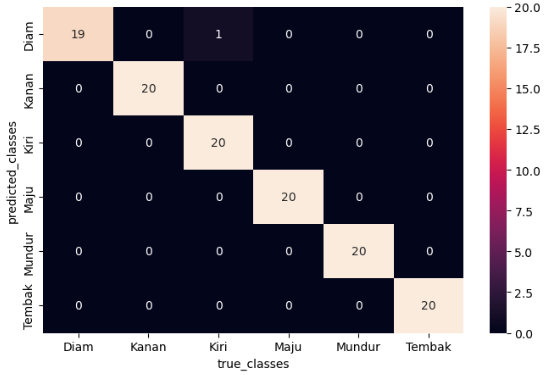
\includegraphics[width=0.4\linewidth]{gambar/cm50.png} \\
        a. Jarak 30cm & b. Jarak 50cm \\ 
        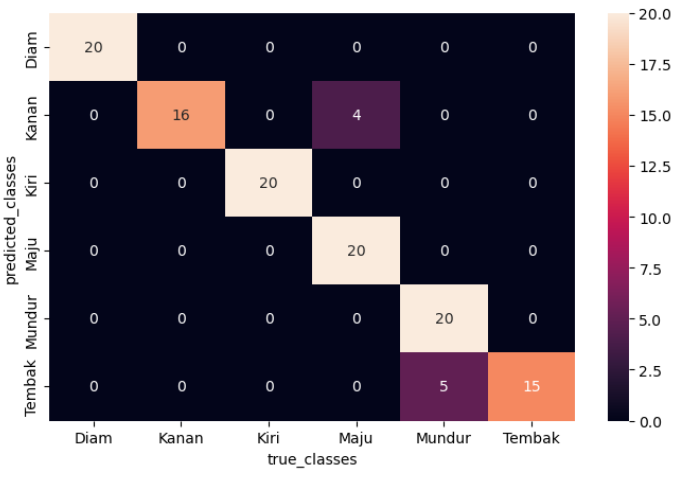
\includegraphics[width=0.4\linewidth]{gambar/cm80.png} & 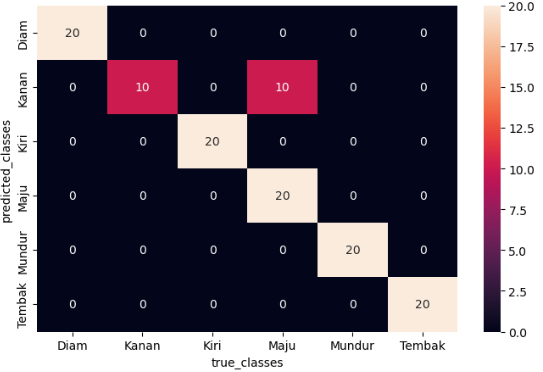
\includegraphics[width=0.4\linewidth]{gambar/cm100.png} \\
        c. Jarak 80cm & d. Jarak 100cm
      \end{tabular}
      \centering
      \caption{Pengujian \emph{Confussion Matrix} pada jarak tertentu}
      \label{fig:confusionmatrixjarak}
  \end{figure}
  

  % \item Pengujian intensitas cahaya \\
  % Pengujian intensitas cahaya 
  % \item Pengujian sudut kamera \\
\end{enumerate}